\documentclass[
aps,
prl,
reprint,
showpacs,
]{revtex4-1}
\pdfoutput=1

\usepackage{booktabs}
\usepackage{graphicx}
%\usepackage{preprintcover}
\usepackage{multirow}
\usepackage{subfigure}
\usepackage[hyperindex,breaklinks,hidelinks,colorlinks,allcolors=blue]{hyperref} 

%\PreprintCoverPaperTitle{\protect\input{00_Title.tex}}
%
%\PreprintIdNumber{CERN-PH-EP-2014-047}
%
%\PreprintJournalName{Phys. Rev. Lett.}
%
%\PreprintCoverAbstract{\input{00_Abstract}}

\begin{document}

\title{A Monoenergetic Neutrino Source from Kaon Decay at Rest}

\author{Rory S. Fitzpatrick}
%\collaboration{ATLAS Collaboration}

\begin{abstract}
\noindent Reconstructing neutrino energies is a challenge for all neutrino experiments with any source. We examine the advantages of identifying monoenergetic neutrino sources such as decay-at-rest kaons and pions and discuss a recent observation of 236 MeV muon neutrinos in the MiniBooNE detector and the prospects of future measurements. 
\end{abstract}

%\pacs{13.38.Dg}

\maketitle

Typically, neutrino experiments can only reconstruct neutrinos energies with resolution $\Delta E/E \sim 25\%$. 

\begin{figure}[h]
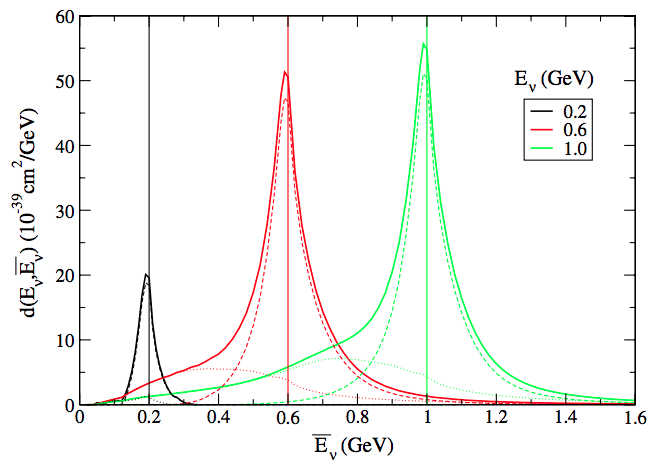
\includegraphics[width=.95\linewidth]{img/nuRes} 
\caption{Simulated neutrino energy resolutions at 200 MeV, 600 MeV and 1 GeV. Figure 1 in \cite{martini}.}
\label{fig:ereco}
\end{figure}

Charged kaons decay to a muon and muon neutrino ($K^+ \rightarrow \mu^+ \nu_\mu$) 63.6\% of the time. Since this is a two-body decay, if the kaon decays at rest, simple kinematics dictate that the outgoing muon neutrino must have an energy of 236 MeV. Monoenergetic neutrino sources are unprecedented and a kaon decay at rest source could vastly improve our understanding of neutrino-nucleus interactions and provide a standard candle for energy reconstruction in the 100s of MeV energy regime \cite{kdar2}. This neutrino could also be used as a probe for a high-$\Delta m^2$ oscillation \cite{kdar1, kdar3}, for precision measurements of the strange spin component of the nucleon $\Delta s$ \cite{kdar2} and as a possible signature for dark matter annihilation in the sun \cite{kumar, kumar2}.

Pion decay at rest also results in a monoenergetic neutrino source at 29.8 MeV, but this is below the charged current threshold and thus a less effective probe.

It is difficult to model the outgoing muon spectrum when a KDAR neutrino interacts because the energy region is such that the impulse approximating breaks down. Figure \ref{fig:landscape} shows the predictions from several neutrino generators and illustrates the degree to which the spectrum remains elusive. A measurement of the spectrum could constrain the model space and improve our understanding of neutrino-nucleus interactions.

\begin{figure}[h]
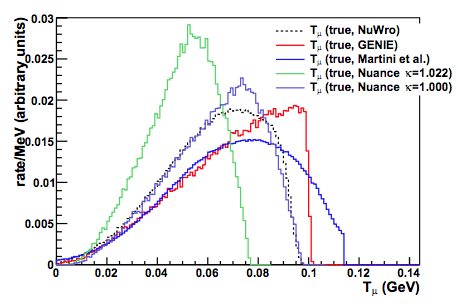
\includegraphics[width=.95\linewidth]{img/kdarLandscape} 
\caption{A number of predictions for the outgoing muon energy when a 236 MeV muon neutrino interacts in the MiniBooNE detector (carbon target). Clearly, there are dramatic variations in both shape and normalization predicted by the different generators.}
\label{fig:landscape}
\end{figure}

kdar at miniboone

\begin{figure}[h]
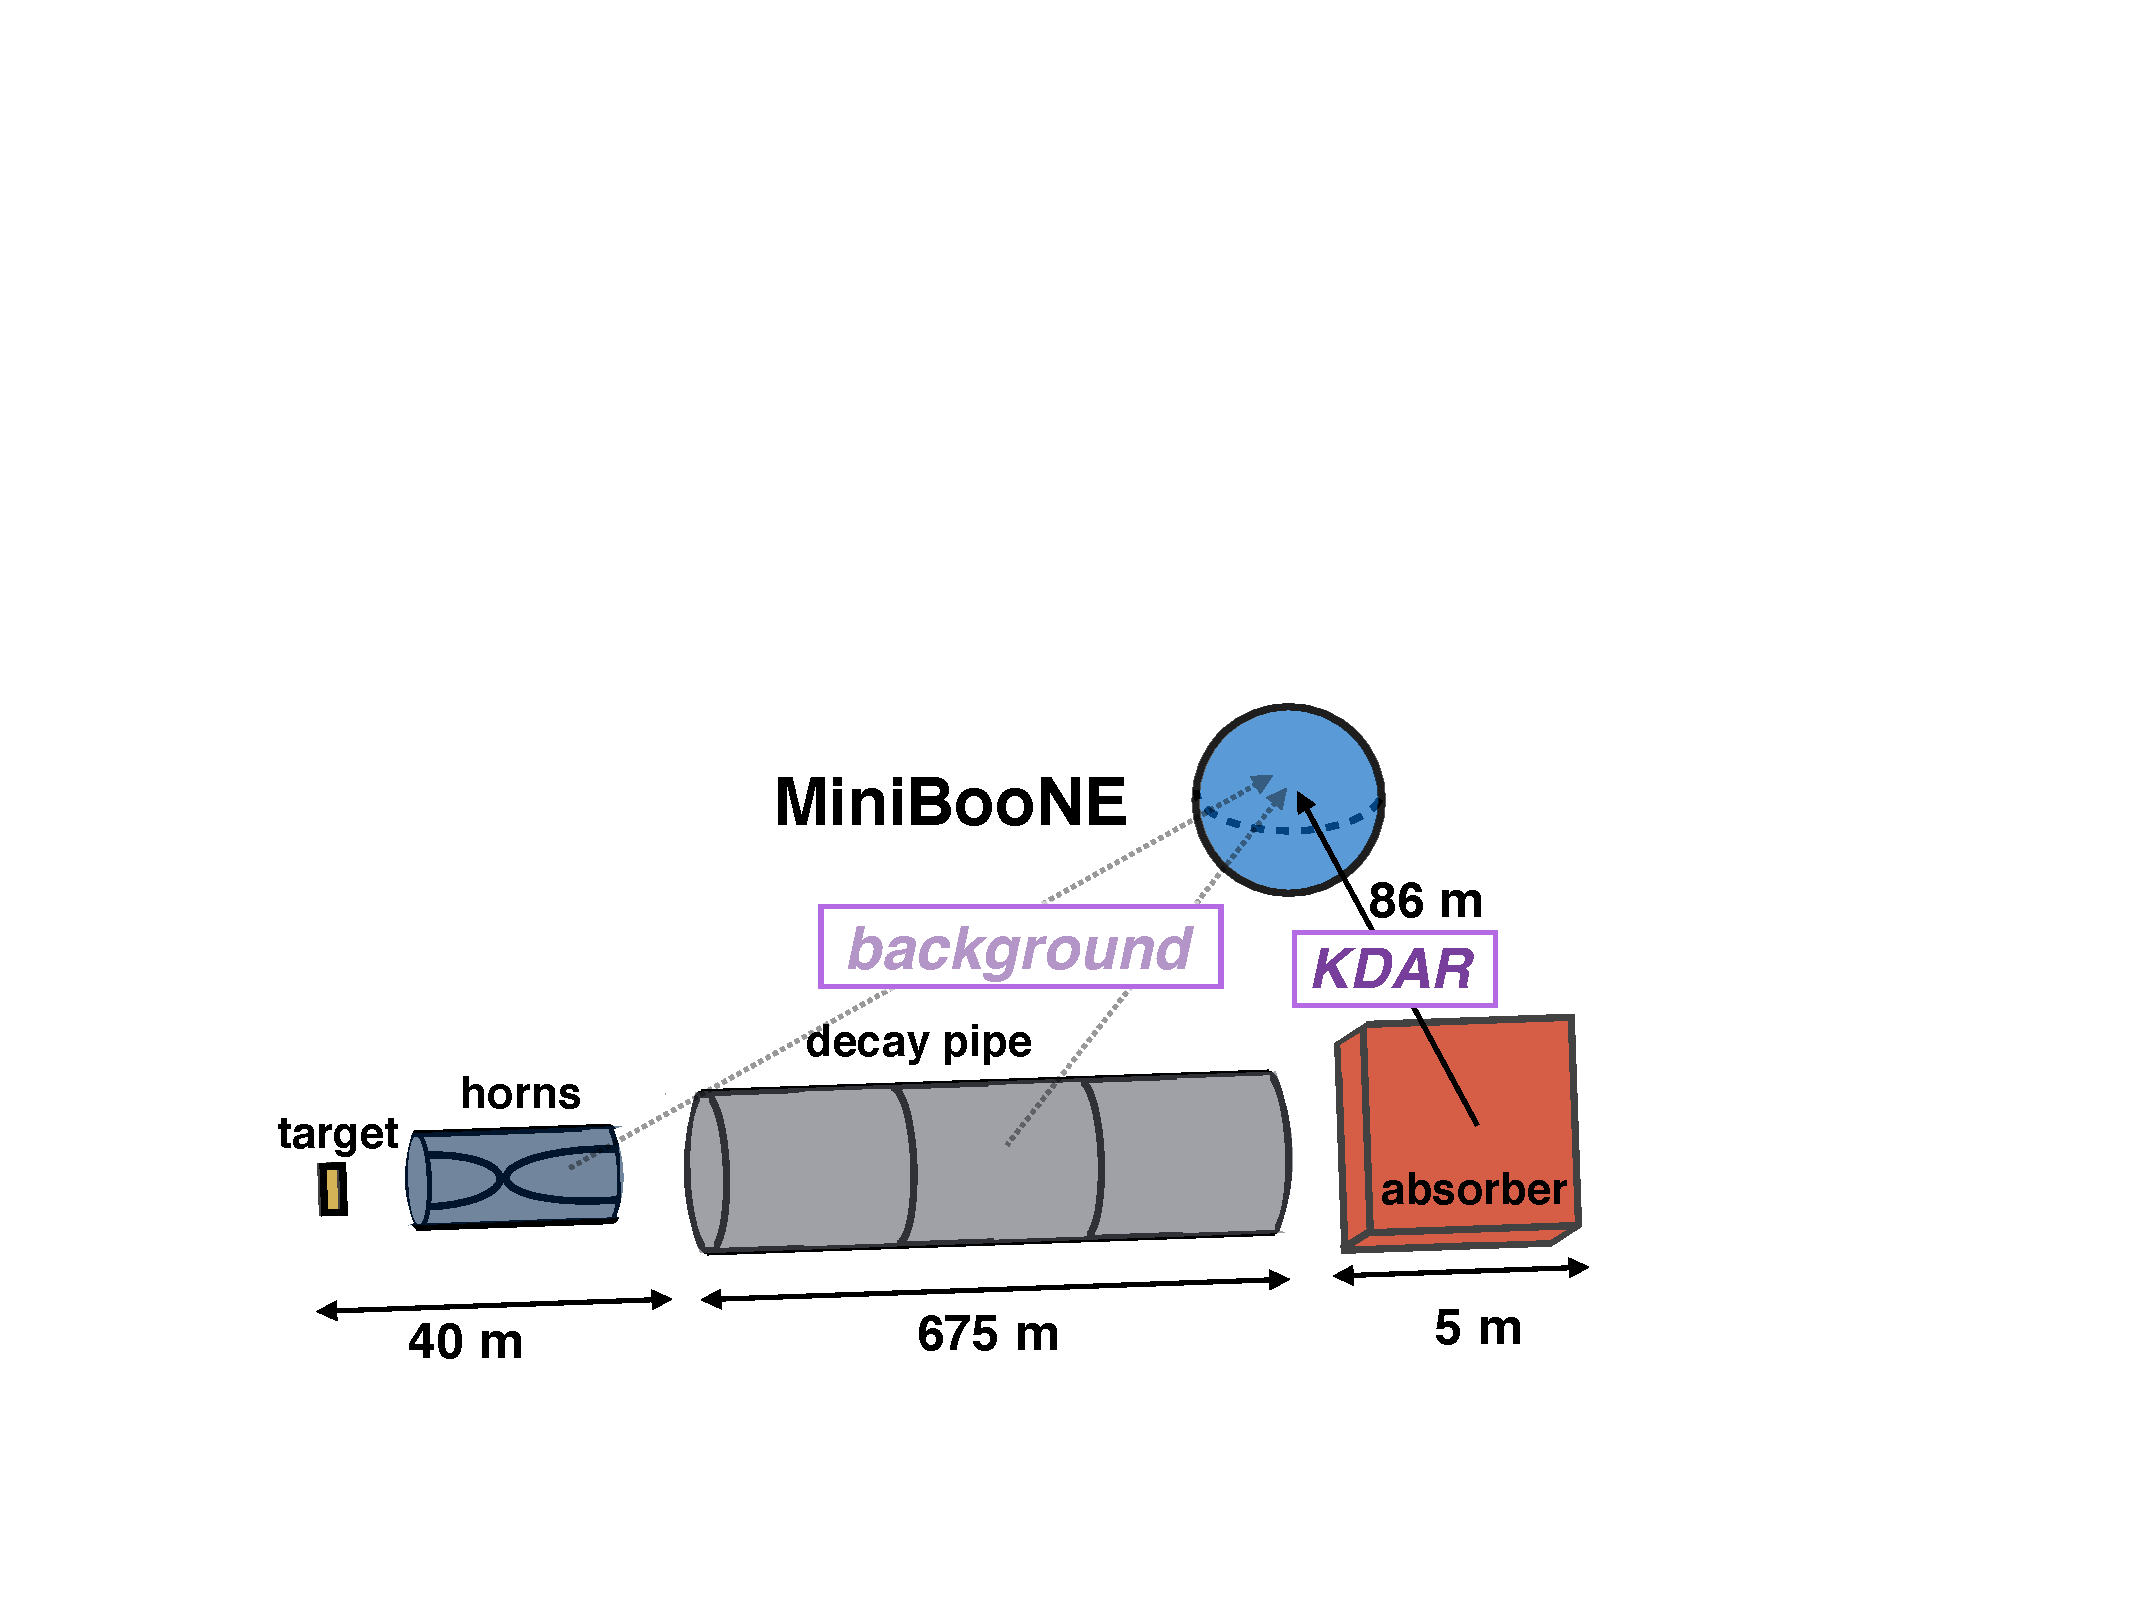
\includegraphics[width=.95\linewidth]{img/beamSchematic} 
\caption{CAPTION}
\label{fig:beam}
\end{figure}

\begin{figure}[h]
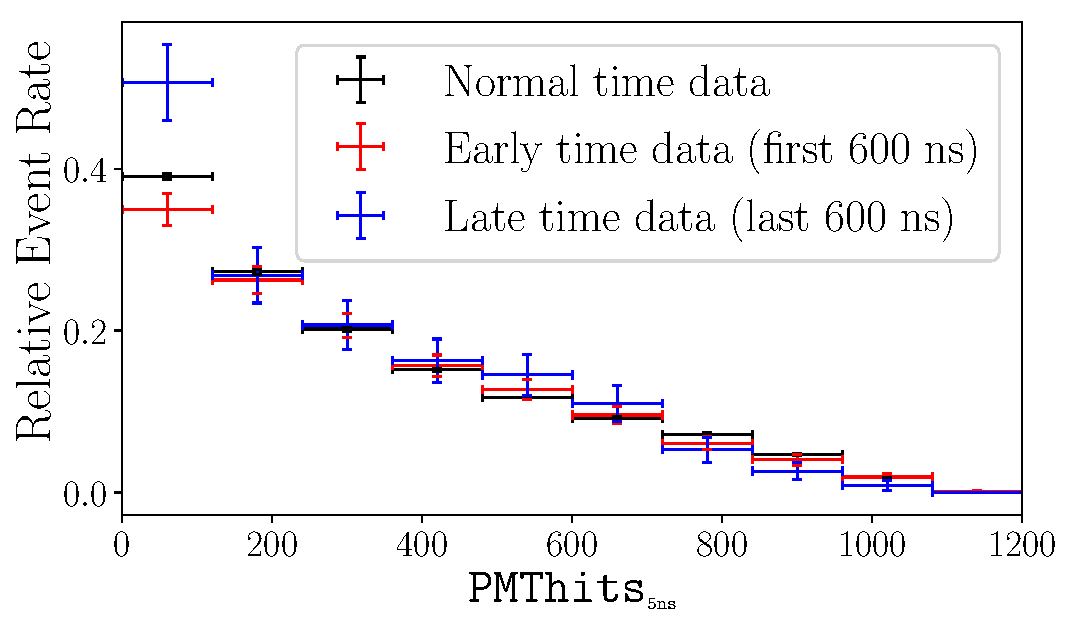
\includegraphics[width=.95\linewidth]{img/observation} 
\caption{CAPTION}
\label{fig:obs}
\end{figure}



future of kdar neutrinos

The error on the MiniBooNE result is statistics dominated and cannot rule out any current models. However, this measurement will be further constrained by a measurement from MicroBooNE, which can also detect KDAR neutrinos from the NuMI beam dump, and by the JSNS$^2$ experiment. The expected rates for all current and upcoming KDAR results are listed in Table \ref{tab:exp}.

\begin{table*}
  \label{tab:exp}
  \begin{ruledtabular}
  \newcommand{\twrw}[1]{\multirow{2}{*}{#1}}
  \begin{tabular}{lccc}
  Experiment & Exposure (POT) & Distance from source (m) & 236 MeV $\nu_\mu$ events \\
    \hline
MiniBooNE & $2.62\times 10^{20}$ (1 year) & 86 m& $3500\pm1500$ \\
MicroBooNE & $1.2\times 10^{21}$ (2 years) & 102 m & 2300 \\
JSNS$^2$ & $1.125\times 10^{23}$ (3 years) & 24 m  & 30-60k \\

  \end{tabular}
  \end{ruledtabular}
    \caption{A summary of experiments that can detect KDAR neutrinos and the event rates expected.}
\end{table*}

\begin{thebibliography}{9}

\bibitem{kdar1}
J. Spitz,  Phys.\ Rev.\  D {\bf 85} 093020 (2012).
 

\bibitem{kdar3}
S. Axani, G. Collin, J.M. Conrad, M.H. Shaevitz, J. Spitz, T. Wongjirad, Phys. Rev. D \textbf{92} 092010 (2015).

\bibitem{kdar2}
J. Spitz, Phys.\ Rev.\  D {\bf 89} 073007 (2014).

\bibitem{kumar}
C. Rott, S. In, J. Kumar, and D. Yaylali, J. of Cosmology and Astroparticle Physics \textbf{11} 039 (2015).

\bibitem{kumar2}
C. Rott, S. In, J. Kumar, and D. Yaylali, arXiv:1710.03822 [hep-ph].

\bibitem{crpa}
V. Pandey, N. Jachowicz, T. Van Cuyck, J. Ryckebusch, and M. Martini, Phys. Rev. C \textbf{92} 024606 (2015).

\bibitem{martini}
M. Martini, M. Ericson, and G. Chanfray, Phys. Rev. D \textbf{87} 013009 (2013).

\end{thebibliography}

\end{document}
